Sequence diagrams will begin in the following page.

\begin{figure}
\centering
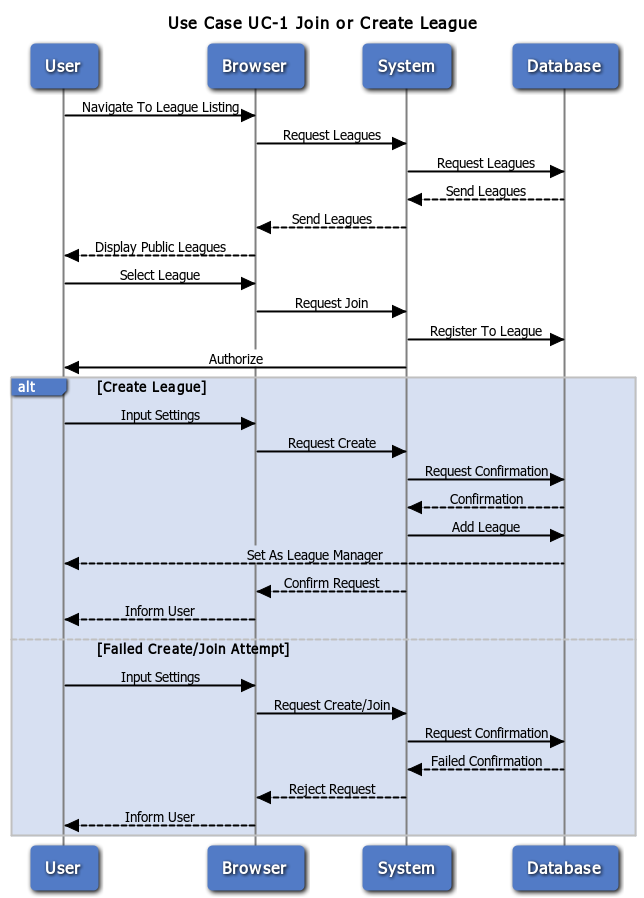
\includegraphics[width=5.5in]{./Diagrams/SystemSequenceDiagrams/uc1.png}
\caption{Sequence Diagram for UC-1 on page \pageref{UC-1}}
\end{figure}

\begin{figure}
\centering
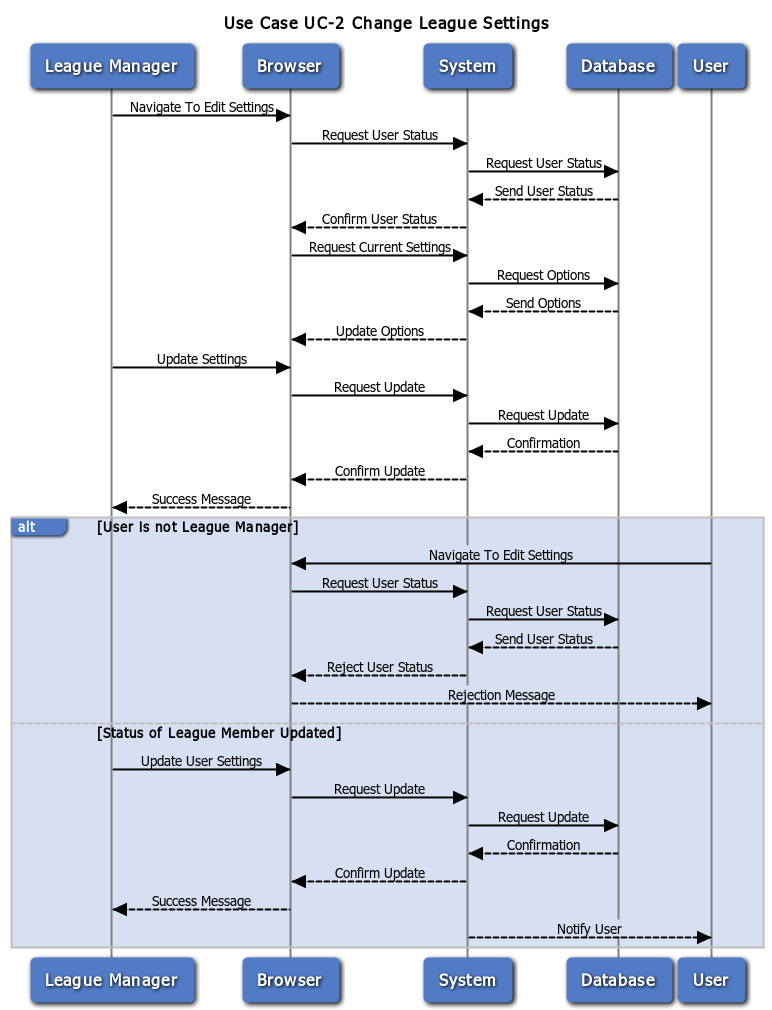
\includegraphics[width=5.5in]{./Diagrams/SystemSequenceDiagrams/uc2.png}
\caption{Sequence Diagram for UC-2 on page \pageref{UC-2}}
\end{figure}

\begin{figure}
\centering
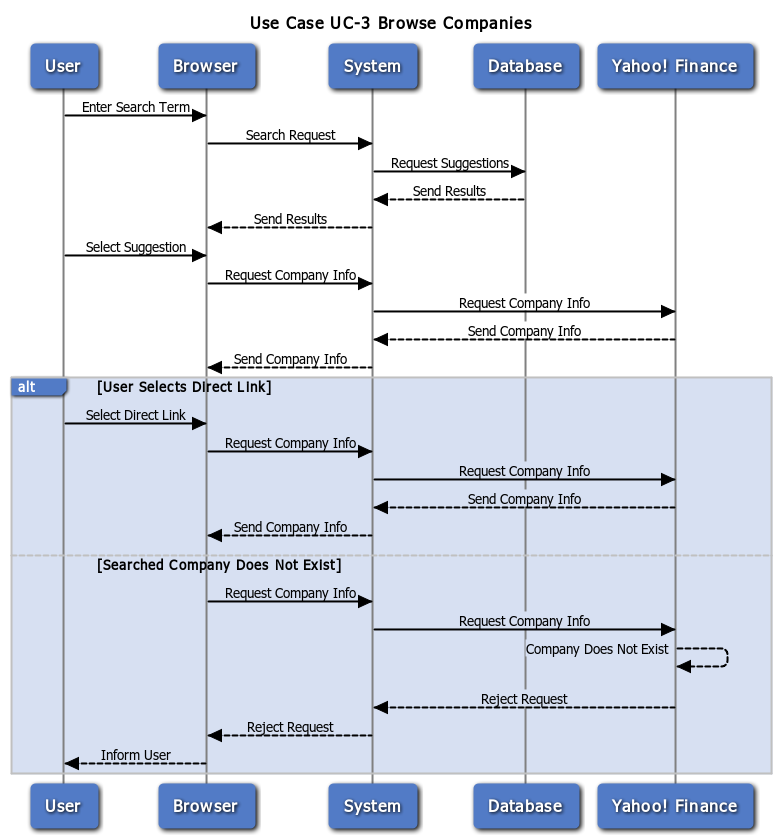
\includegraphics[width=5.5in]{./Diagrams/SystemSequenceDiagrams/uc3.png}
\caption{Sequence Diagram for UC-3 on page \pageref{UC-3}}
\end{figure}

\begin{figure}
\centering
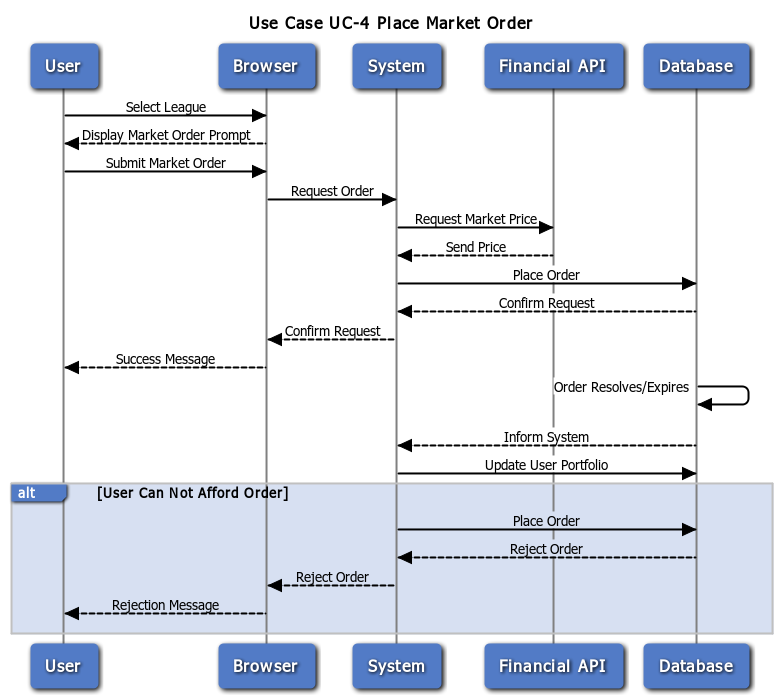
\includegraphics[width=5.5in]{./Diagrams/SystemSequenceDiagrams/uc4.png}
\caption{Sequence Diagram for UC-4 on page \pageref{UC-4}}
\end{figure}

\begin{figure}
\centering
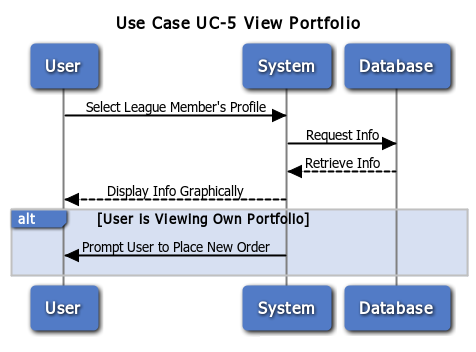
\includegraphics[width=5.5in]{./Diagrams/SystemSequenceDiagrams/uc5.png}
\caption{Sequence Diagram for UC-5 on page \pageref{UC-5}}
\end{figure}

\begin{figure}
\centering
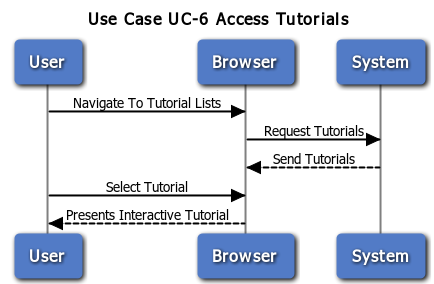
\includegraphics[width=5.5in]{./Diagrams/SystemSequenceDiagrams/uc6.png}
\caption{Sequence Diagram for UC-6 on page \pageref{UC-6}}
\end{figure}

\begin{figure}
\centering
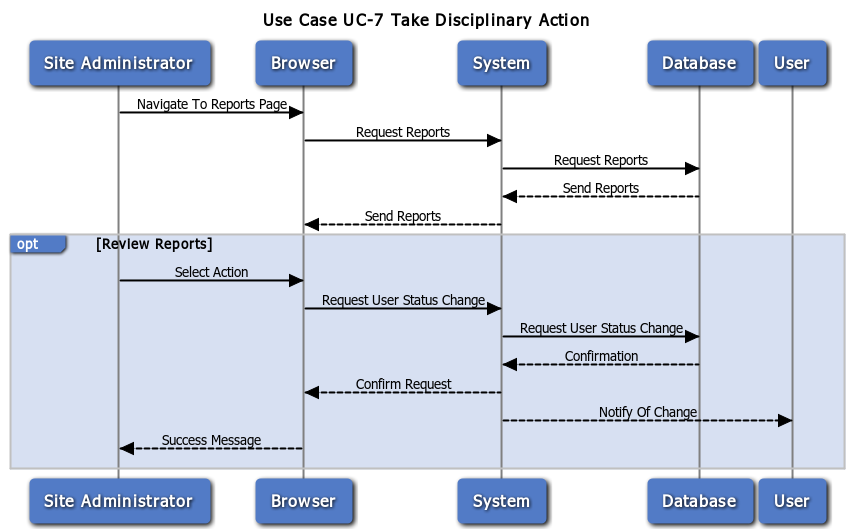
\includegraphics[width=5.5in]{./Diagrams/SystemSequenceDiagrams/uc7.png}
\caption{Sequence Diagram for UC-7 on page \pageref{UC-7}}
\end{figure}
